\documentclass[a4paper]{article}
\usepackage{xgreek}
\usepackage{xltxtra}
\usepackage{graphics}
\setlength{\topmargin}{0in}
\setlength{\oddsidemargin}{0in}
\setlength{\evensidemargin}{0in}
\setlength{\textheight}{9in}
\setlength{\textwidth}{6.25in}
\setmainfont[Mapping=tex-text]{GFS Didot}

\begin{document}
\section{Κονσόλα Διαχείρισης Κόμβων}
Η κονσόλα διαχείρισης κόμβων του ScorpioFS είναι μια λειτουργία με την οποίο
μπορούμε να διαχειριστούμε κόμβους του δικτύου απομακρυσμένα. Όπως βλέπουμε και
από το Σχήμα \ref{fig:topology}, το δίκτυο αποτελείται από τους Chord κόμβους με ένα
proxy server και το σύστημα με το ScorpioFS και τη κονσόλα διαχείρισης.\\

\begin{figure}[tbh]
\centering
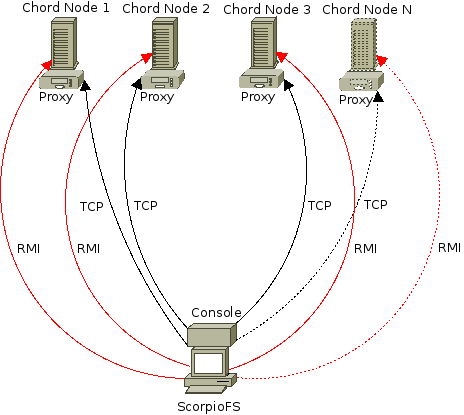
\includegraphics[scale=0.75]{images/scorpio_console.png}
\caption{Τοπολογία δικτύου κόμβων}
\label{fig:topology}
\end{figure}

Το πρωτόκολλο επικοινωνίας μεταξύ του ScorpioFS συστήματος και των κόμβων του
δικτύου για ανταλλαγή δεδομένων είναι το \emph{RMI} ενώ για την επικοινωνία της
κονσόλας διαχείρισης και των Proxy server είναι \emph{TCP}. Η επικοινωνία μέσω
\emph{RMI} γίνεται από τη θύρα 6788 ενώ η επικοινωνία μέσω \emph{TCP} γίνεται
από τη θύρα 6789. Κάθε εν δυνάμει Chord κόμβος τρέχει τον proxy server του, ακόμα και αν δεν είναι ακόμα μέλος του δικτύου. Μέσω της κονσόλας διαχείρισης δίνουμε εντολές που μεταφέρονται σύμφωνα με ένα συγκεκριμένο πρωτόκολλο στον proxy server του κάθε Chord node και αυτός με τη σειρά του αναλαμβάνει για την κλήση των κατάλληλων μεθόδων. Οι εντολές που υποστηρίζει η κονσόλα διαχείρισης είναι οι παρακάτω:
\begin{itemize}
    \item \textbf{node create IP\_ADDR[:port]} -- Δημιουργία ενός νέου Chord
κόμβου στο δίκτυο.
    \item \textbf{node stop IP\_ADDR[:port]} -- Κλείσιμο του συγκεκριμένου
κόμβου.
    \item \textbf{node stat IP\_ADDR[:port]} -- Παραγωγή στατιστικών για το
συγκεκριμένο κόμβο, τη συγκεκριμένη ώρα.
    \item \textbf{node alive IP\_ADDR[:port]} -- Έλεγχος αν ένας κόμβος είναι
ενεργός.
    \item \textbf{node list} -- Προβολή όλων των ενεργών κόμβων στο δίκτυο.
    \item \textbf{scorpiofs mount ARGS} -- Ξεκίνημα της υπηρεσίας ScorpioFS στο
τοπικό μηχάνημα.
    \item \textbf{scorpiofs unmount} -- Σταμάτημα της υπηρεσίας ScorpioFS.
    \item \textbf{terminate} -- Σταμάτημα όλων των Chord κόμβων στο δίκτυο με
έξοδος από την κονσόλα διαχείρισης.
    \item \textbf{help} -- Προβολή βοήθειας.
\end{itemize}

Το πρωτόκολλο επικοινωνίας μεταξύ της κονσόλας διαχείρισης και του proxy κάθε
Chord node ορίζεται από τα παρακάτω:

\begin{center}
\begin{tabular}{|c|c|}
\hline
\textbf{Mnemonics} & \textbf{Code}\\
\hline
\hline
NODE\_CREATE & 0\\
\hline
NODE\_STOP & 1\\
\hline
NODE\_STAT & 2\\
\hline
NODE\_ALIVE & 3\\
\hline
NODE\_LIST & 4\\
\hline
SCORPIOFS\_MOUNT & 5\\
\hline
SCORPIOFS\_UNMOUNT & 6\\
\hline
TERMINATE & 7\\
\hline
CHORD\_PORT & 6788\\
\hline
PROXY\_PORT & 6789\\
\hline
\end{tabular}
\end{center}
\end{document}
